As the user interface shows (Figure~\ref{usermanual_UI}), there are several buttons and radio buttons to control and call different function of this retrieval system: 

\begin{enumerate}[1.]
\item ``LoadMesh'': loads the 3D model
\item ``AddNoise'': adds noise to the model
\item ``Denoise'': applies bilateral filter for 3D denoising
\item ``Rotate\_X (Y/Z)'': rotates the model around X (Y/Z) axis 
\item ``Normalize'': normalizes the model
\item ``Rasterize'': rasterizes the model into voxels 
\item ``BatchTransform'': batch transforms the models in the database to descriptors and save them into descriptors database
\item ``Retrieve'': compares the similarity between current descriptors with all the descriptors in the database
\item ``Candidate1 (2/3/4/5/6)'': shows the candidates with high similarities.
\item ``PointCloud'': shows the model in point-cloud mode.
\item ``Polygon'': shows the model in polygon mode.
\end{enumerate}

For testing purpose and viewing the intermediate processes, it is recommended to press buttons in this sequence: LoadMesh, (AddNoise,Denoise,Rotate\_X (Y/Z)),  Normalize, Rasterize, Retrieve, Candidate1 (2/3/4/5/6).

\begin{figure}[h]
\centering
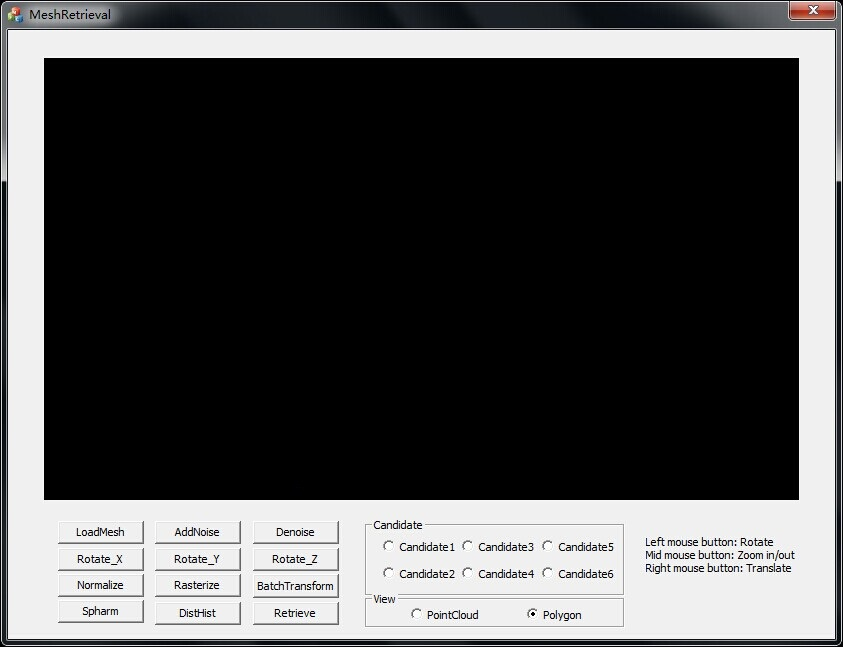
\includegraphics[width=0.7\linewidth]{UI}
\caption{User Interface} \label{usermanual_UI}
\end{figure}